% !TEX root = praca.tex

\chapter{Środowisko eksperymentalne}
\label{cha:srodowiskoEksperymentalne}

Autonomiczny system kompletacji zamówień wymagał stworzenia odpowiedniego środowiska, w którym pojazd mógłby się poruszać. Należało opracować odpowiednią strukturę przestrzenną sklepu. Zdecydowano się na sklep z trzema głównymi alejkami, do których można wejść od góry dołu i środka XD

%--------------------------------------------------------------------------

\section{Rzeczywista plansza}
\label{cha:plansza}
W celu uproszczenia procesu testowania zdecydowano się na wykonanie papierowej makiety odwzorowującą możliwe trasy przejazdu w sklepie w zmniejszonej skali. Papierowa plansza miała wymiary 480 x 280 cm, a możliwe trasy zostały przedstawione za pomocą czarnej taśmy. Dodatkowo na planszy wyznaczono punkty decyzyjne robota w postaci punktów przecięcia, które oznaczono poprzez poprzeczne ułożenie taśmy.

\begin{figure}[htbp]
    \centering
    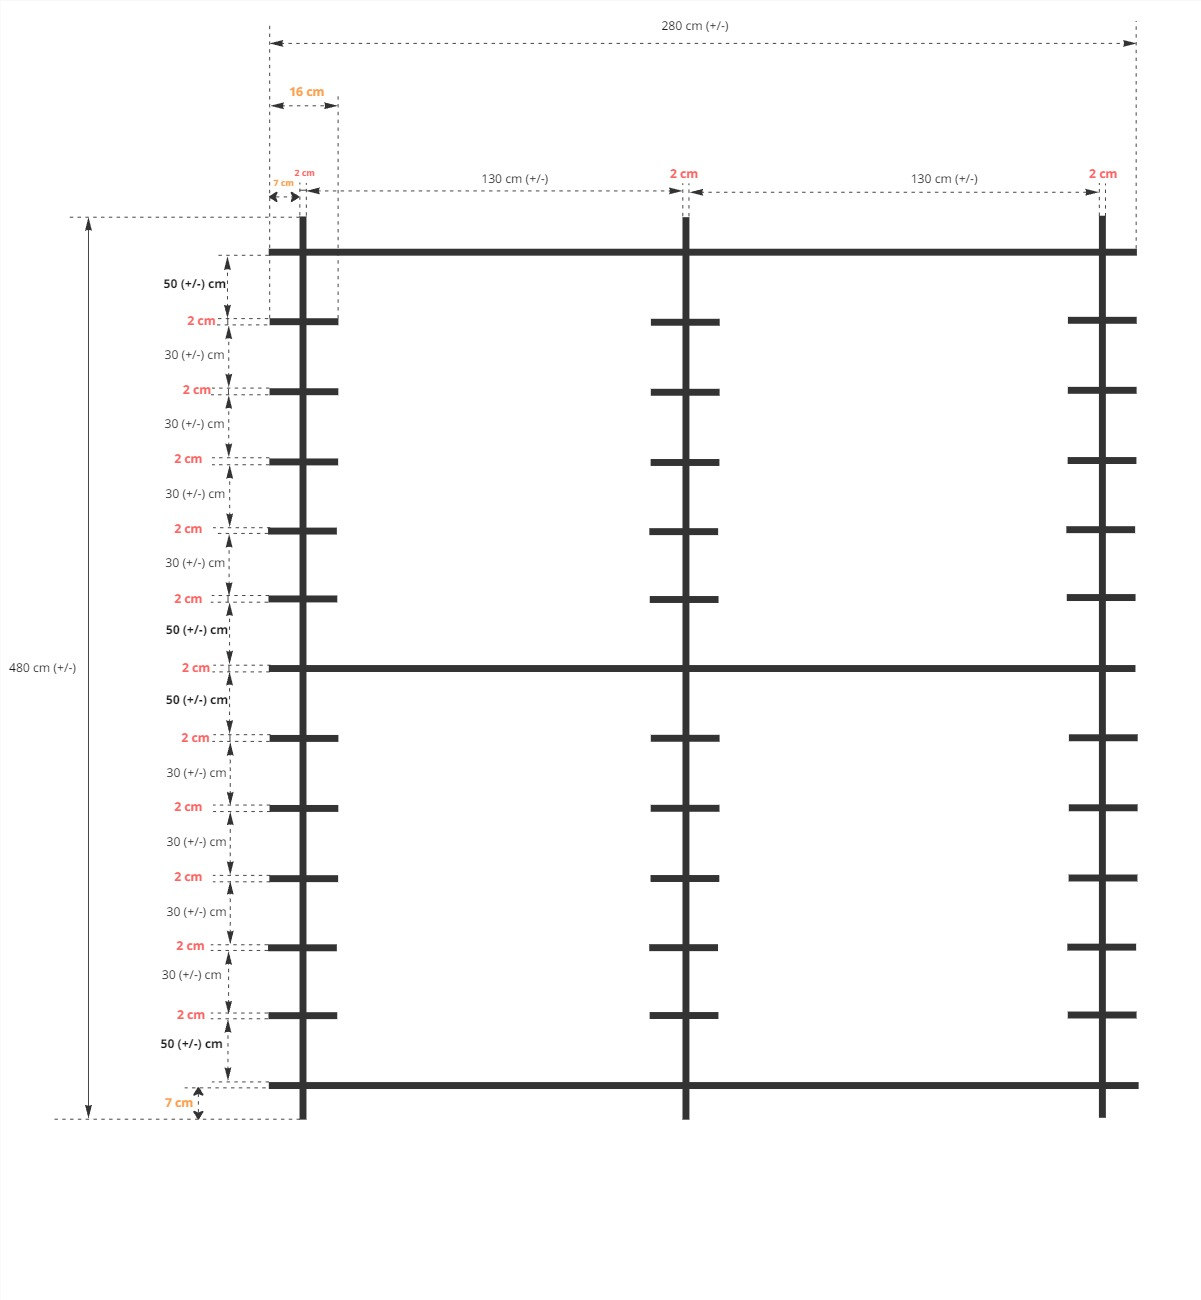
\includegraphics[width=0.8\textwidth]{images/shopModel.jpg}
    \caption{Model tras przejazdu w sklepie}
    \label{fig:pathModel}
\end{figure}

%--------------------------------------------------------------------------

\section{Graf}
\label{cha:graf}

Algorytmy TSP opierają się na znalezieniu minimalnego cyklu Hamiltona w grafie (?), dlatego należy przedstawić strukturę tras w sklepie za pomocą grafu. Każdy punkt przecięcia na planszy odpowiada wierzchołkowi w grafie, a w celu łatwiejszej identyfikacji zostały oznaczone jako współrzędne kartezjańskie. Dodatkowo odległości między punktami przecięć zostały odwzorowane w grafie jako wagi krawędzi.
Ponieważ w pracy zdecydowano się na jeden pojazd, graf jest nieskierowany, a trasy nie są podwajane w celu ustalenia 2 kierunków jazdy. 

\begin{figure}[htbp]
    \centering
    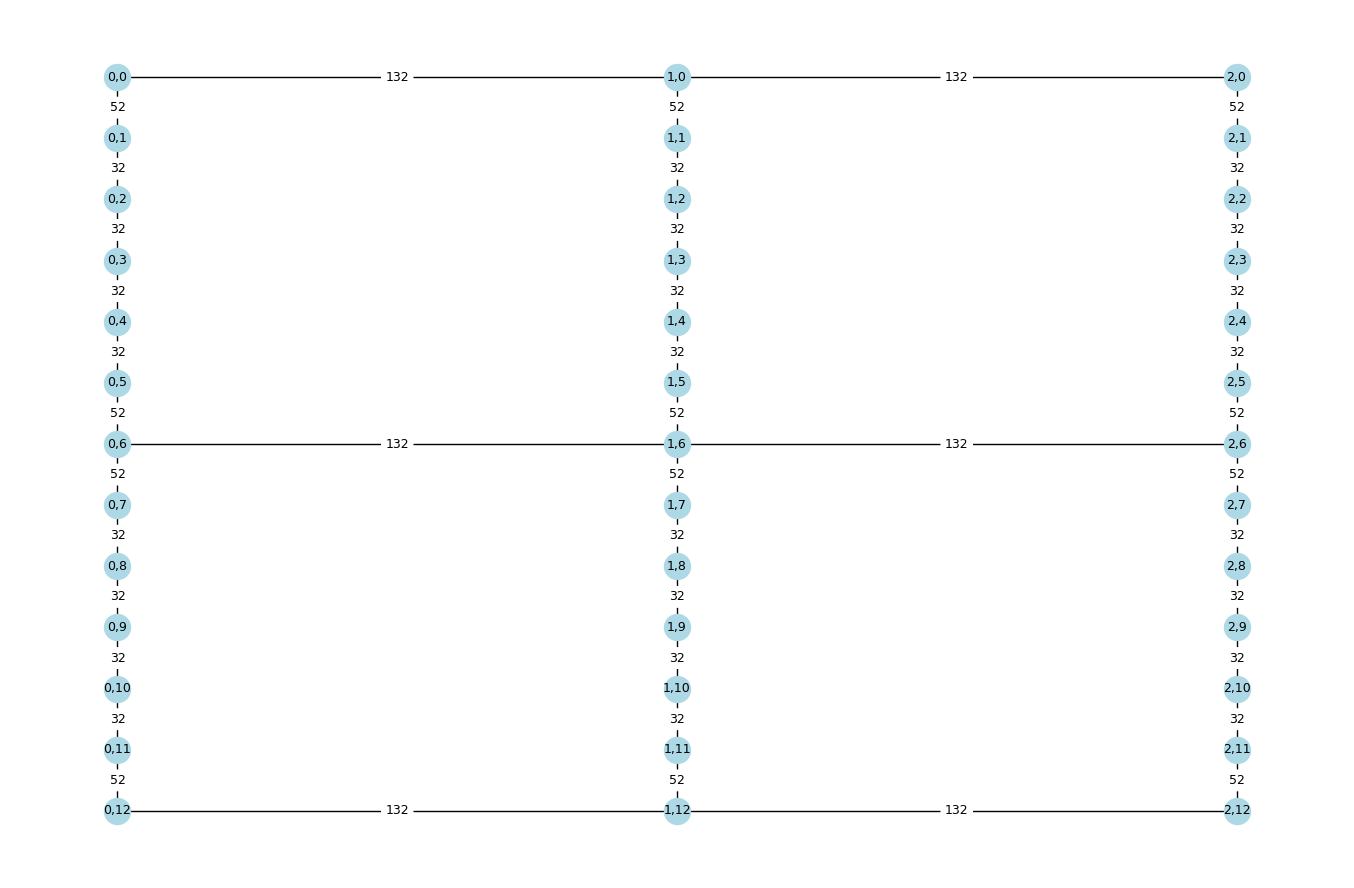
\includegraphics[width=1\textwidth]{images/graph.png}
    \caption{Makieta odwzorowujący strukturę przestrzenną sklepu}
    \label{fig:graph}
\end{figure}
